% No 'submit' option for the problems by themselves.
%\documentclass{harvardml}
% Use the 'submit' option when you submit your solutions.
\documentclass[submit]{harvardml}

\usepackage{url}
\usepackage{bbm}

% Put in your full name and email address.
\name{Nicolas Drizard}
\email{nicolasdrizard@g.harvard.edu}

% You don't need to change these.
\course{CS265}
\assignment{Project Update}
\duedate{March 13, 2016}

% Useful macros
\newcommand{\bw}{\boldsymbol{w}}
\newcommand{\distNorm}{\mathcal{N}}
\newcommand{\given}{\,|\,}
\newcommand{\ident}{\mathbb{I}}
\newcommand{\btheta}{\boldsymbol{\theta}}
\newcommand{\bz}{\boldsymbol{z}}
\newcommand{\balpha}{\boldsymbol{\alpha}}
\newcommand{\bbeta}{\boldsymbol{\beta}}
\usepackage{amsmath}
\usepackage{hyperref}
\usepackage{graphicx}
\usepackage[toc,page]{appendix}
\usepackage{url, enumitem}
\usepackage[procnames]{listings}

% Some useful macros.
\newcommand{\R}{\mathbb{R}}
\newcommand{\E}{\mathbb{E}}
\newcommand{\var}{\text{var}}
\newcommand{\cov}{\text{cov}}
\newcommand{\N}{\mathcal{N}}
\newcommand{\ep}{\varepsilon}

\theoremstyle{plain}
\newtheorem{lemma}{Lemma}

\usepackage{float}
\floatplacement{figure}{H} % force figures to be placed always at defined position!
\begin{document}

\part*{CS 265 Development Project: Plan}

\subsection*{Introduction}

This project aims to build a data structure providing low-cost indexing for a file experiencing a high rate of record inserts/deletes over an extended period: Log-Structured Merge-tree (LSM-tree). LSM-Trees operates on batch for the inserts/updates, cascading the changes from its first compononent $C_0$ (memory based) to one or more larger (disk-based).


\subsection*{Data Structure}

One of the first design questions concerns the data structure used in the two types of components ($C_0$ the entry component in memory, and $C_i$ on disk). An intuitive choice for $C_0$ is an array as we don't need to keep it sorted, we just append each entry to it. The deeper components need an index-based structure. My first approach is to use a sorted array at each level. The data structure is a key-values store. To minimize the number of scan during the merges and the reads I store in two different arrays the keys and the values.

Once the data structure of each component is defined, we need to store also metadata of our LSM Tree. These metadata will contain the following information:
\begin{itemize}
	\item number of element (long Ne);
	\item number of components (long Nc);
	\item array of ratios from one component to the next one (int ratios[]);
	\item array of pointers to each level ( int *c[Nc])
\end{itemize}

The last element can also be a linked list of pointers in the case we do not know in advance the number of components. We can choose to expand indefinitely the number of components or to choose the last component as indefinitely growing. I will first implement the latter and may benchmark the two options afterwards.


\subsection*{Operations}

The LSM Tree need to support INSERT, READ, UPDATE and DELETE. We will treat similarly the INSERT, UPDATE and DELETE operations.

\paragraph{INSERT UPDATE DELETE}
These operations aim to add/retrieve to the Tree a tuple (key, value). The key may be already stored but the overall approach is the same. We insert them in the unsorted $C_0$ component and then they will go through each component until the last non empty one to be stored, if not already stored. If on the way the same key is found then its value get updated. For the deleted operation, the value of the key will take a special value corresponding to an empy value. We will delete it from its cell in the corresponding component.

We need to define the merging strategy that enables to cascade the changes from one component to the next one by batch.

\begin{figure}[H]
\begin{center}
    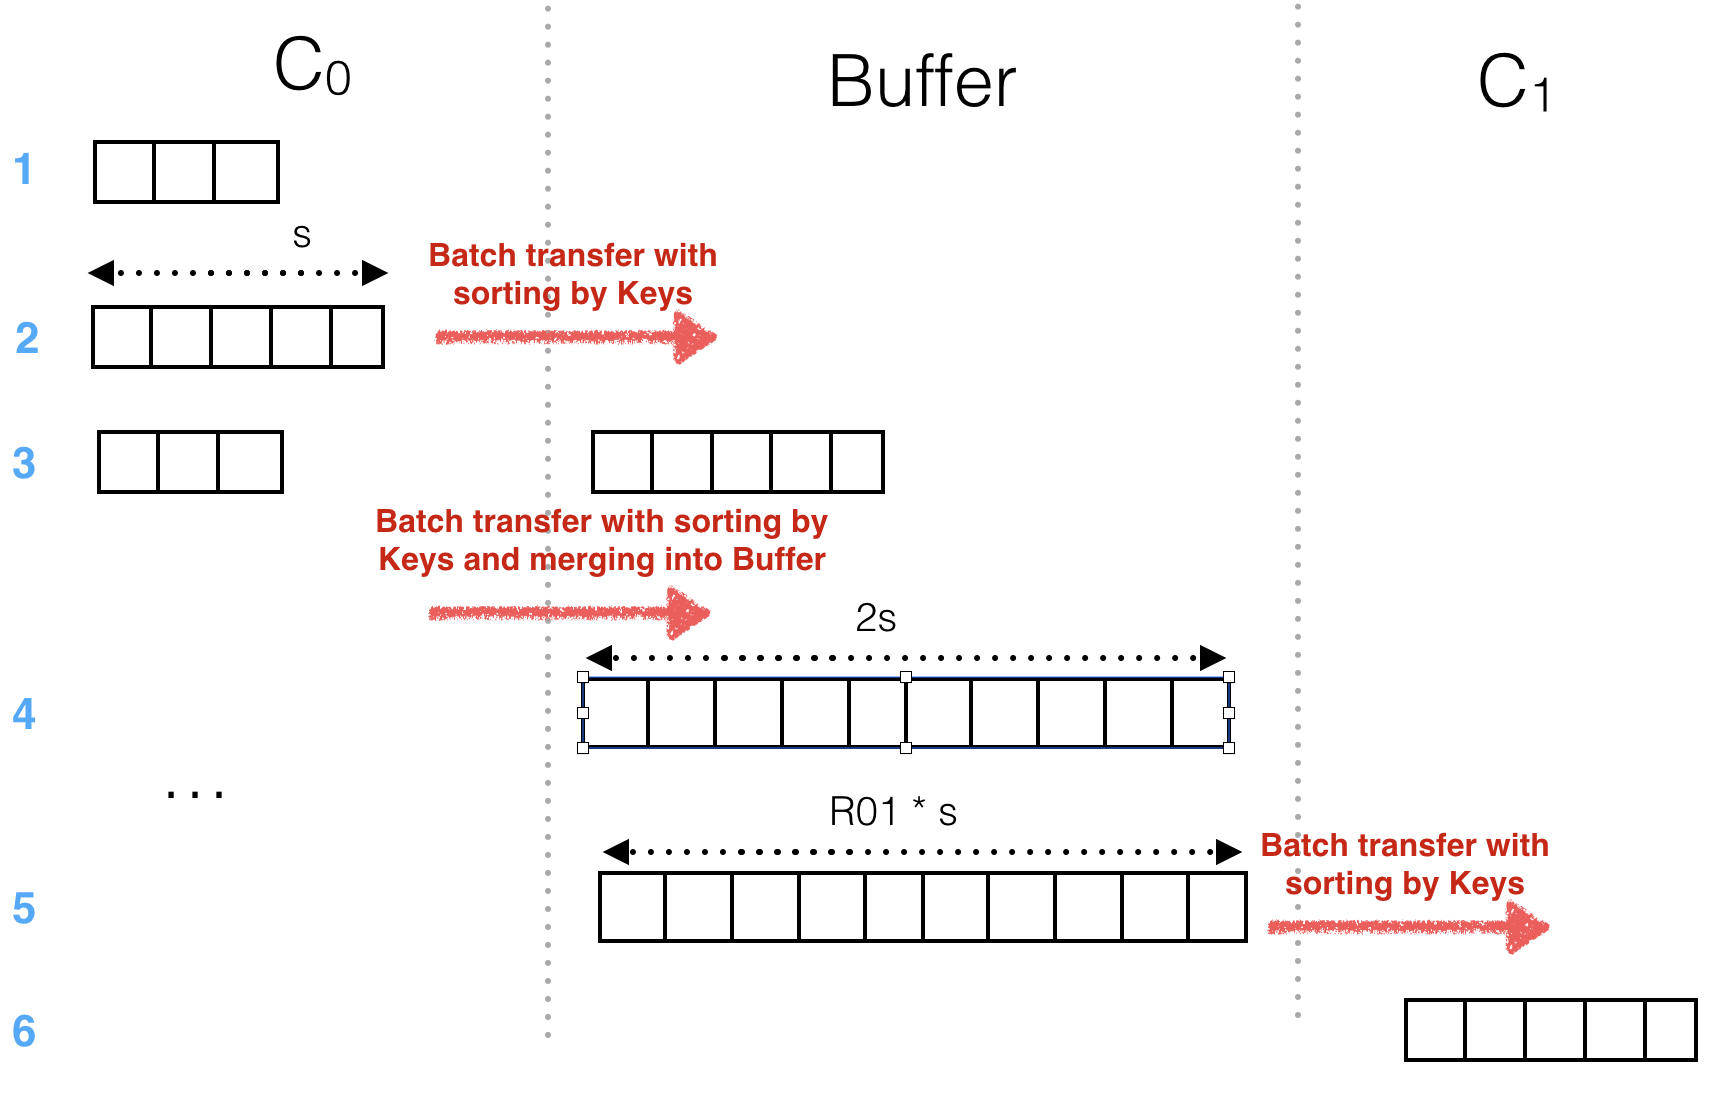
\includegraphics[width=0.6\textwidth]{merge}
    \caption{Merging Strategy}
\end{center}
\end{figure}

I provide a figure to illustrate my merging strategy. First, I use a buffer between $C_0$ and $C_1$ but then between $C_i$ and $C_{i+1}$ for $i \neq 0$ it's the same behavior than between the Buffer and $C_1$. $C_0$ is kept unsorted and we just append elements to it. When it reaches its threshold size s, we transfer it to the buffer while sorting it. If the buffer is empty, we fill it, otherwise we merge the incoming array with the existing one inside the buffer to have it sorted. If the resulting array reaches the Buffer threshold, which is the product between the size s and the ratio of size between $C_0$ and $C_1$ $R_{0,1}$, we transfer it entirely to the next component and act in the same way we transfered from $C_0$ to the Buffer. Generally, the threshold for component $i$ is $R_{i-1,i} \times s_{i-1}$. This approach enables to implement right away a multi-components architecture for the LSM.

\paragraph{READ}

When reading, we need to search in each component. First, we do a linear scan in $C_0$ and then we look into each deeper component with a binary search.


\subsection*{Storage}

This part presents briefly the storage of the different objects. Each deep component $C_i$ for $i \neq 0$ is stored on disk in 2 files, one for the keys, one for the values. The names and pointers to these two files are stored in the metadata in the array of the components. The component $C_0$ and the buffer are kept on memory and saved on disk if we interrupt the script. The metadata are stored in memory and on a separate file on disk if interruption.

\subsection*{Benchmark}

First, we have to evaluate the influence of different parameters: threshold size of $C_0$ and the ratios. I will use benchmarks involving about 1 million operations, in a skewed case and in a random one, and report the running time to compare these parameters.

Another tuning may be done with the merging approach. Instead of keeping only one array at each component level, we could keep more and merge them when we reach a given size. This should increase the searching time but decrease the insertion time as we merge less often. We need to confirm this intuition and evaluate the workload tailored to each of the two scenarios.

\subsection*{Future Work}

Once a functional version of this LSM Tree will be implemented. I will improve it by taking advantage of a multicore execution. The reading operations could be easily run on parallel as we need to search at each component. However, the insert operations are already optimized by the nature of this multi-components Tree and need to be done sequentially so may work need to be done to come up with an eventual parallel implementation of that part.

Concurrently, another data structure may be tried for the deeper component. I may try a B-tree structure as it's commonly used to stores index. I will compare it to the sorted arrays for different kind of workloads.

\end{document}
